\hypertarget{src_HLS_registerAllocation_page_register_definition}{}\section{Register allocation problem defition}\label{src_HLS_registerAllocation_page_register_definition}
The {\bfseries storage value insertion} phase inserts additional nodes in the scheduled data flow graph. Each edge that crosses a cycle step boundary represents a value that has to be stored somewhere. The storage allocation function can therefore be defined as the following transformation\+:

Given a scheduled data flow graph $G(V_o,E,C)$, the {\bfseries storage value insertion} is a transformation $G(V_o,E,C)\rightarrow (V_o\cup V_s,E',C)$, which adds storage value $v\in V_s$ to the graph such that all edges $e\in E$ which cross a cycle step boundary are connected to a storage value.

The {\bfseries register allocation} problem can be formulated as the allocation of a storage module $m\in M_s$ for each storage value $v\in V_s$\+:

{\bfseries Register allocation}\+: the {\itshape register allocation} function $\psi : V_s\rightarrow \Pi(M_s)$, identifies the storage module holding a value from the set $V_s$

The binding information is needed for evaluating and/or performing the register optimization. Therefore, the accurate estimation of the number of registers requires both scheduling and binding.\hypertarget{src_HLS_registerAllocation_page_compatibility_graph}{}\section{Compatibility graph definition}\label{src_HLS_registerAllocation_page_compatibility_graph}
The main task to provide good solutions to the {\bfseries register allocation} problem is the procedure used to recognize the overlapping of the life time intervals. Since a register is needed for the values alive between two control steps, the analysis can be easily performed on state transition graph (see \hyperlink{src_HLS_controller_stg}{Finite State Machine}). In fact, a vertex in this graph represent all operations executed in a control step. The value that will be further needed will be alive across the edges outcoming from this vertex. Besides, an edge represents the changing from a control step to the next one, so the values alive between two control steps are the values alive on this edge. The dataflow analysis, presented by Appel, allows to compute, for each edge, which are the variables alive. These variables will be the vertices of a {\itshape conflict graph}, that is a graph so defined\+:
\begin{DoxyItemize}
\item the vertices are the variables that have to be stored into a register (since that are alive between two control steps)
\item an edge connects two variables if they are alive in the same moment, that is they are alive on the same edge.
\end{DoxyItemize}

The resulting conflict graph is minimal with respect to number of conflicting variables (i.\+e. the number of edges in the graph). In a such way, the solution to register allocation problem will use the minimum number of registers. The problem can be formulated as a clique-\/covering problem (search of largest cliques into the compatibility graph, complementary to the conflict one) and it can be easily resolved with an heuristic vertex coloring on conflict graph. An heuristic coloring assigns a different color to source and target of each edge. So variables alive in the same moment will be connected all together by conflict edges, so they will be differently colored. Since each color used will represent a different register in the final design, the variables will be assigned, as requested, to different registers. When variables are not alive together, there are no conflict edges so it can happen that the algorithm assigns to the variables the same color. It means that they could share the same register, in fact the values are not alive in the same moment.\hypertarget{PandA_DOC_intro}{}\section{Introduction}\label{PandA_DOC_intro}
Into data flow graph, each edge represents a data value. If the value crosses a cycle step boundaries, it has to be stored into a register.~\newline
 For example, in the data flow graph below, the edges from {\itshape n1} to {\itshape n3}, from {\itshape n2} to {\itshape n4} and from {\itshape n3} to {\itshape n4}, cross the low boundary of control step 1 and control step 2. Each of this edge represents a storage value and so, it has to be assigned to a register. 
\begin{DoxyImageNoCaption}
  \mbox{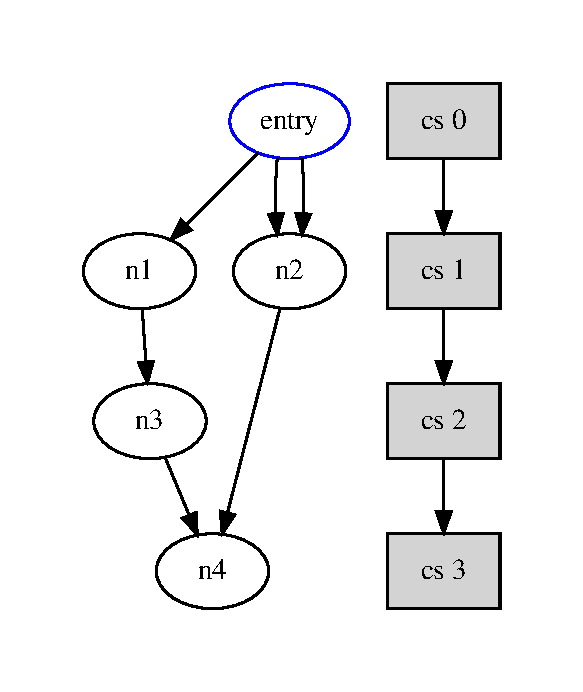
\includegraphics[width=\textwidth,height=\textheight/2,keepaspectratio=true]{dot_inline_dotgraph_21}}
\end{DoxyImageNoCaption}
 This can be considered the first and simpler approach to register allocation problem. This section has the goal to exploit some properties of the problem and try to reduce the number of storage modules. It is organized as follow. The subsection \hyperlink{src_HLS_registerAllocation_page_definition}{Principles of register allocation} explains and defines the problem in other to get a more reasonable approach. Subsection \hyperlink{src_HLS_registerAllocation_page_traditional}{Traditional approach to register allocation problem} overviews the classical approach to register allocation and \hyperlink{src_HLS_registerAllocation_page_pandaApproach}{PandA\textquotesingle{}s approach to register allocation} defines the approach adopted and implemented into PandA framework. Finally, subsection \hyperlink{src_HLS_registerAllocation_page_algorithms}{Algorithms overview} shortly defines algorithms implemented into register\+Allocation class.\hypertarget{src_HLS_registerAllocation_page_definition}{}\section{Principles of register allocation}\label{src_HLS_registerAllocation_page_definition}
The register allocation problem is defined as finding a solution to the register allocation function $ \psi : V_s \rightarrow \Pi( M_s ) $, that identifies the storage module (like registers and register files) holding a value from the set $ V_s $ of values that have to be stored. A storage module has to be assigned to each storage value. If the register allocation problem is considered in isolation, the goal is to minimize the number of storage modules. Every storage value is labeled with the variable it belongs to using a function $ var: V_s \to LV $ where $LV$ is the set of variables from the language.~\newline
 The function $ \omega : V_s \to C $ determines for each storage value the cycle step in which it is written.~\newline
 The function $ \rho : V_s \to \Pi(C) $ determines the set of cycle steps in which the storage value is read. The function $ P: V_s \to C $, determines the last cycle step in which the storage value $ v \in V_s$ is read. Thus, $ P(v) = max(\rho(v)) $.~\newline
 A storage value {\itshape v} that is written in state $ \omega(v) $ and read for the last time in the state $ P(v) $ is called {\itshape life} in the interval $ lt(v) = [\omega(v), P(v)] $. The interval will be called {\itshape lifetime} ({\itshape interval}) of a storage value {\itshape v}. The requirement to keep storage values from one variable together is modeled by a set of lifetimes assigned to each variable $ u \in LV $. The function $ LT(u) $ describes this set of lifetimes\+: $ LT(u) = \{lt(v_s)|var(v_s) = u, u \in LV\} $\hypertarget{src_HLS_registerAllocation_page_compGraph}{}\subsection{The compatibility and conflict graphs}\label{src_HLS_registerAllocation_page_compGraph}
Usually, from an examination of the control/data flow graph, it can be derived a {\itshape conflict} {\itshape graph} $ G_s(V_s,W) $ (also called {\itshape interference} {\itshape graph}), where nodes $ V_s $ are the storage value to be stored, and edges W are pairs of values that cannot be assigned to the same storage module because they are alive at the same time. This means that the storage values that are adjacent in $ G_s(V_s,W) $ cannot be stored in the same register because their interval life overlap. Concluding, two vertices are joined by an edge if they are in conflict. The complement of a conflict graph will be called {\itshape compatibility} {\itshape graph}.~\newline
~\newline
 Edges $\bar{W}$ of the {\itshape compatibility} {\itshape graph} $ \bar{G}_s(V_s,\bar{W}) $ (e.\+g., the complement of the conflict graph $ G_s(V_s,W) $ described above) are defined as follow\+:~\newline
~\newline
 $ \bar{W}=\lbrace (v_{i},v_{j}) \mid \ll \omega(v_{i}),P(v_{i}) \gg \parallel \ll \omega(v_{j}),P(v_{j}) \gg = false\rbrace $~\newline
~\newline
 and $V_s$ is the set of the storage values; $\omega(v)$ and $P(v)$ are the write and last read cycle steps and the operator $||$ returns true if two intervals overlap and return false otherwise\+:~\newline
~\newline
 $\ll x_1, y_1 \gg || \ll x_2, y_2 \gg =$ $ \\false,\ if\ y_1<x_2\vee y_2<x_1\\true,\ otherwise$ ~\newline
~\newline
 This means that storage values that are adjacent in $G_s(V_s,W)$ can be stored in the same register without overwriting each others values.\hypertarget{src_HLS_registerAllocation_page_traditional}{}\section{Traditional approach to register allocation problem}\label{src_HLS_registerAllocation_page_traditional}
A clique covering algorithm, applied to compatibility graph, groups the values in such a way that all values that belong to the same clique can be stored in the same register. ~\newline
 A heuristic algorithm for clique covering of compatibility graph is the Tseng\textquotesingle{}s algorithm. The clique covering is done using a heuristic that first combines those nodes having the most neighbors in common. To break a tie also the number of excluded edges from the combination is calculated. One edge is selected from this set $W''$. A new vertex $v_a$ represents the union of the cliques of $v_1$ and $v_2$. All excluded edges are removed from the graph and $v_a$ is connected to the remaining edges of $v_1$. Finally, $v_1$ and $v_2$ are removed from the graph.~\newline
 Solving the general clique problem will attempt to minimize the number of registers needed to store all the variables. Method register\+Alg\+::clique\+\_\+cover() implements the Tseng\textquotesingle{}s clique cover algorithm.~\newline
~\newline
 However, there are special cases in which more efficient algorithms may be used, as explained into \hyperlink{src_HLS_registerAllocation_page_algorithms}{Algorithms overview}.~\newline
 It\textquotesingle{}s known that finding a clique covering in a graph $G$ is the dual problem of finding a coloring in the complement graph $\overline{G}$,so method register\+Alg\+::coloring() provides a way to solve register allocation problem by conflict graph coloring as these graph are one the complement of each other by definition and they are both provided from compatibility\+Graph objects.\hypertarget{src_HLS_registerAllocation_page_pandaApproach}{}\section{Pand\+A\textquotesingle{}s approach to register allocation}\label{src_HLS_registerAllocation_page_pandaApproach}
\hypertarget{src_HLS_registerAllocation_page_use_RFSDG}{}\subsection{Use of Reducted S\+D\+G Graph}\label{src_HLS_registerAllocation_page_use_RFSDG}
What said in the previous section could be considered as a conservative approach. In fact, with a further and careful analysis, the conflict graph can be pruned by unuseful constraints (e.\+g. unuseful interference edges) due to false conflicts among variables. So, storage values that were considered conflicting before, now can become compatible and so the number of storage modules can be further reduced. \textbackslash{} In particular, the analysis focuses on the fact that more than one mutual exclusive control flow can exist in the behavioural description\+: this means that a pair $ (v_i,v_j) $ of storage values can holds the same register (in spite of their interval life overlap or not) if $ v_i,v_j $ belong to paths that are in mutual exclusion each other. \textbackslash{} So, in order to perform this analysis, it can be useful to use a different flow graph representation, the Reduced System Dependence \hyperlink{structGraph}{Graph} with information about Feedback edges (the R\+F\+S\+DG \hyperlink{structGraph}{Graph}), that contains all the information you may need afterwards about data and control dependences. This graph represents the transitive reduction of the usual System Dependence \hyperlink{structGraph}{Graph} (the S\+DG graph); it\textquotesingle{}s used at this step because it shows a complete and minimum representation of all control/data flows.\hypertarget{src_HLS_registerAllocation_page_data}{}\subsection{Dataflow Analysis}\label{src_HLS_registerAllocation_page_data}
Dataflow analysis, based on Appel\textbackslash{}\textquotesingle{}s approach, has been quite modified to obtain better result in a multi-\/flow problem, such as a usual D\+FG is.~\newline
 First step is usual dataflow analysis, where live variables are computed for each vertex, to get information about liveness. Liveness information ({\itshape live-\/in} and {\itshape live-\/out}) can be calculated from {\itshape use} and {\itshape def} as the following dataflow equations shows\+: ~\newline
~\newline
 $ in[n] = use[n] \bigcup (out[n] - def[n]) $ ~\newline
 $ out[n] = \bigcup_{s \in succ[n]} in[s] $ ~\newline
~\newline
 These dataflow equations for liveness analysis mean that\+:
\begin{DoxyItemize}
\item If a variable is {\itshape use\mbox{[}n\mbox{]}}, than it is {\itshape live-\/in} {\itshape at} node {\itshape n}. That is, if a statement uses a variable, the variable is live on entry to the statement.
\item If a variable is $ live-in $ at node $ n $, than it is $ live-out $ at all nodes in $ pred[n] $.
\item If a variable is $ live-out $ at node $ n $, an not in $ def[n] $, than the variable is also $ live-in $ at $ n $. That is, if someone needs the value of $ a $ at the end of statement $ n $, and $ n $ does not provide that value, then $ a $\textbackslash{}\textquotesingle{}s value is needed even on entry to {\itshape n}.~\newline
 A solution to these equations can be found by iteration. $ in[n] $ and $ out[n] $ are initialized to the empty set \{\}, then the equations are repeatedly treated as assignment until a fixed point is reached.~\newline
 The convergence of this algorithm can be significantly speeded by ordering the nodes properly; this can be done easily by postorder ordering. ~\newline
~\newline
 After that, unuseful informations have to be cleaned. They are because the graph is a multiflow one and so vars can flow through wrong paths (they would not reach their defs). So the second step is a forward analysis, where each var definition is propagated up to the end of interval life, so when the variable is $ live-in$ and not $ live-out$ at the operation vertex or when there is a new definition of the same variable in the vertex. Merging nodes having to be take carefully\+: they also merge variable definitions. ~\newline
 Now, if a variable is live into a node and it has not any defs, it means it is a variable in a wrong path and so it can be eliminated from the computation. This forward analysis is computed until fixed point has been reached and it ensures a right and meanful computation of liveness analysis.
\end{DoxyItemize}\hypertarget{src_HLS_registerAllocation_page_cgcreation}{}\subsection{Conflict graph creation}\label{src_HLS_registerAllocation_page_cgcreation}
After dataflow analysis, conflic graph can be created. In graph creation, each edge into the control flow graph is taken into account. If source vertex and target one are scheduled into different control step, it means that a register is needed for each variable living out from the source vertex to keep value alive until target one will use them. So a conflict edge can be set between each pair of variable in a such situation\+: they cannot use the same register module. However, it is a conservative approach. Now, some improvements implemented into the proposed solution have been explained.~\newline
 This algorithm is able to detect $ alias $ variables. In fact, theorically, each vertex can execute only one operation and so store only one result. Multi-\/definitions are allowed only by using statements like as\+: ~\newline
~\newline
 $ a = b = c + d $ ~\newline
~\newline
 In this way, variable {\itshape a} and variable {\itshape b} are different ones but they contain the same value, so they can share the same register. In proposed solution, they can be detected because definitions have been forwarded. So, during the analysis of an edge, if two variables are both alive and definition vertex is the same, they can be considered {\itshape alias} and then there is not conflict between them. ~\newline
~\newline
 There is no conflict also when the defining vertices are in mutual exclusion. In fact, at run-\/time, if a variable is defined by a vertex, the other one will not be defined, so register could be shared between them. ~\newline
 Constants and read input variables doesn\textquotesingle{}t need any register.  pair of variables living togheter and without any of above properties are in conflict. So an edge between them must be added into the conflict graph.\hypertarget{src_HLS_registerAllocation_page_bestalg}{}\subsection{Choose of the Best Algorithm}\label{src_HLS_registerAllocation_page_bestalg}
As shown in Figure \textbackslash{} ref\{fig\+:flowchart\}, there are four main register allocation algorithms. The best one is chosen on the basis of a precise analysis of the topology of the resulting conflict graph. In fact there are special cases in which efficient algorithms may be used.~\newline
 Before describing precisely each algorithm, some definition can be useful\+:
\begin{DoxyItemize}
\item {\itshape I\+N\+T\+E\+R\+V\+AL G\+R\+A\+PH}\+: an undirected graph G is called an interval graph if its vertices can be put into one-\/to-\/one correspondence with a set of intervals of a linearly orders set (like the real line) such that two vertices are connected by an edge of G iff their corresponding intervals have nonempty intersection. An interval graph satisfies the triangulated graph property;
\item {\itshape C\+H\+O\+R\+D\+AL G\+R\+A\+PH}\+: an undirected graph G is called a triangulated graph (or chordal graph) if every cycle of length strictly greater than three possesses a chord;
\item {\itshape C\+Y\+C\+L\+IC G\+R\+A\+PH}\+: an undirected graph G is called a cyclic graph if it contains a cycle.~\newline
 Next subsections specify what are those efficient algorithms named before and what are the special cases in which they may be used.
\end{DoxyItemize}\hypertarget{src_HLS_registerAllocation_page_algorithms}{}\section{Algorithms overview}\label{src_HLS_registerAllocation_page_algorithms}
\hypertarget{src_HLS_registerAllocation_page_lea}{}\subsection{Left Edge Algorithm}\label{src_HLS_registerAllocation_page_lea}
The lifetimes of all values are represented by intervals. The register allocation problem can be viewed as the problem of assigning the intervals to registers along a horizontal line, such that no two intervals in the same register overlap. These intervals can be seen as wires which have to be assigned to tracks (the registers), which will make this problem analogous to the channel routing problem without vertical constraints. A left edge algorithm can be used to solve this problem.~\newline
 ~\newline
 Left edge algorithm $G_s (V_s , W)$ ~\newline
~\newline
 $\\.sort\_values(v\in V_s,\omega (v)); \ \ \ M_s=\emptyset; \\ .\mathbf{foreach} \ v \in \ V_s \ \mathbf{do} \\ .\ \ \ \mathbf{foreach}\ r \in \ M_s\ \mathbf{do} \\ .\ \ \ \ \ \ \ \mathbf{if} \ \omega (v) \ > P(r) \ \mathbf{then} \\ .\ \ \ \ \ \ \ \ \ \ \ \psi(v)=r; \ \mathbf{then} \\ .\ \ \ \ \ \ \ \ \ \ \ P(r)=P(v);\\ .\ \ \ \ \ \ \ \mathbf{endif} \\ .\ \ \ \mathbf{endfor} \\ .\ \ \ \mathbf{if}\ \psi(v)=0 \ \mathbf{then} \\ .\ \ \ \ \ \ \ M_s = M_s \cup \{ r \} ; \ \ \textrm{ / / add new register } \\ .\ \ \ \ \ \ \ \psi(v)=r;\\ .\ \ \ \ \ \ \ P(r)=P(v);\\ .\ \ \ \mathbf{endif} \\ .\mathbf{endfor} $~\newline
 Since the list of registers is pre-\/sorted the check if a new value overlaps with the values in the registers can simply be done by comparing the write time of the value with the last cycle step in which the register is occupied. This cycle step is called the last read step of a register\+: P(r).~\newline
 Sorting is the most complex step in this algorithm and the left-\/edge algorithm can be performed with complexity $O(nlogn)$ where n is the number of values to be stored. Method register\+Alg\+::left\+\_\+edge() implements previously described algorithm.\hypertarget{src_HLS_registerAllocation_page_cgca}{}\subsection{Chordal Graph Coloring Algorithm}\label{src_HLS_registerAllocation_page_cgca}
The left edge algorithm will only guarantee optimality if the life times of all variables can be ordered in a linear fashion. If the data flow graph contains conditionals this may not be the case. When variables are alive across the beginning or ends of conditionals these situations can arise. The lifetimes cannot be represented along a single line but form a tree-\/like structure. The confict register allocation graph is not an interval graph anymore. It can be proved that a graph G is an interval graph, if and only if it does not contain a subgraph which is a so called asteroidal triple. See \mbox{[}1\mbox{]} pag. 16-\/17.~\newline
 Despite the fact that the asteroidal triples cause the conflict graph to be non-\/interval graph, they are still triangular (chordal) graphs. Algorithms exist to efficiently color these graphs. Similar to a left-\/edge algorithm an ordering in which to color the vertices has to be build first. A lexicographic breath first search provides such an ordering. The algorithm returns a sequence of vertices $ \sigma $ which can be used in coloring the graph. Vertices will be picked in order of their maximal labels. Each time a vertex is picked the labels of all its neighbor vertices are updated. The sequence are compared lexicographically. The node sequence returned in $\sigma$ will be a so-\/called perfect vertex elimination scheme.~\newline
 ~\newline
 $\\Lexicographic\ BFS\ G(V,E) \\ \\ .\mathbf{foreach}\ v \in V\ \mathbf{do} \\ .\ \ \ \ label(v)=\emptyset ;\\ .\mathbf{endfor} \\ .\mathbf{for} \ i=|V|\ to\ 1\ \mathbf{do} \\ .\ \ \ \ \mathbf{let}\ v_x \in V\ \textrm{such\ that\ label}(v_x)\ \textrm{is\ maximal};\\ .\ \ \ \ \sigma(i)=v_x;\\ .\ \ \ \ \mathbf{foreach}\ v\in \{Adj(v_x)|\sigma^{-1}(v)=0\}\\ .\ \ \ \ \ \ \ label(v)=label(v)+i;\\ .\ \ \ \ \mathbf{endforeach}\\ .\mathbf{endfor}$

~\newline
 Once such an ordering is obtained a simple modification to the left edge algorithm can be made. All values have to added to the registers in the order prescribed by $\sigma$. The test if a value can be added to a register becomes more complicated than a simple left edge algorithm as one cannot simply test for overlap between the read cycle step of the last value with the new value to be assigned. All values previously assigned to the register have to be checked for overlap. The following algorithm produces the minimal number of registers in case of conflict register allocation graph is a triangular graph. The complexity is O(V+W).~\newline
 $\\ Chordal\ graph\ coloring\ G(V_s,W)\\ \\ .M_s = \emptyset\\ .\mathbf{for}\ k=|V_s|\ to\ 1\ \mathbf{do}\\ .\ \ \ \ v=\sigma(k);\\ .\ \ \ \ \mathbf{foreach}\ r \in M_s\ \mathbf{do}\\ .\ \ \ \ \ \ \ \ \mathbf{if} \not \exists v_s \in r\ \textrm{such that } lt(v_s)||lt(v)=true\ \mathbf{then} \\ .\ \ \ \ \ \ \ \ \ \ \ \ \psi(v)=r;\\ .\ \ \ \ \ \ \ \ \mathbf{endif}\\ .\ \ \ \ \mathbf{endfor}\\ .\ \ \ \ \mathbf{if}\ \psi(v)=0\ \mathbf{then}\\ .\ \ \ \ \ \ \ \ M_s=M_s \cup \{r\};\ \ \textrm{ / / new register}\\ .\ \ \ \ \ \ \ \ \psi(v)=r;\\ .\ \ \ \ \mathbf{endif}\\ .\mathbf{endfor} $

~\newline
 Method register\+Alg\+::chordal\+Coloring() implements the previus chordal graph coloring preceded by the lexicographic breath first search to get the $\sigma$ node order.\hypertarget{src_HLS_registerAllocation_page_craa}{}\subsection{Cyclic Register Allocation Algorithm}\label{src_HLS_registerAllocation_page_craa}
{\itshape Cyclic Register Allocation Algorithm} is the best algorithm to apply when the conflict graph is a cyclic graph, but only when there is almost one cycle of length strictly greater than three. This is due to the fact that if the conflict graph is a cyclic graph but every cycle of length strictly greater than three possesses a chord, this means that the graph is a chordal graph and so one of the two previous algorithm are applied.\hypertarget{src_HLS_registerAllocation_page_references}{}\section{References}\label{src_HLS_registerAllocation_page_references}
\mbox{[}1\mbox{]} L. Stok, \char`\"{}\+Data path synthesis\char`\"{}, {\itshape Integration}, {\itshape V\+L\+SI} {\itshape journal}, Vol.\+18, pp.\+1-\/71, June 1994.

\mbox{[}2\mbox{]} Y.\+L. Lin, \char`\"{}\+Recent Developments in High-\/\+Level Synthesis\char`\"{}, {\itshape A\+CM} {\itshape Trans}. {\itshape Design} {\itshape Automation} {\itshape of} {\itshape Electronics} {\itshape Systems}, vol. 2, pp. 2-\/21, January 1997.

\mbox{[}3\mbox{]} A. W. Appel, \char`\"{}\+Modern Compiler Implementation in Java\char`\"{}, {\itshape Cambridge} {\itshape University} {\itshape Press}, pp. 1-\/548, 1998.

\mbox{[}4\mbox{]} R. Shamir, \char`\"{}\+Advanced Topics in Graph Algorithms\char`\"{}, {\itshape Notes} {\itshape of} {\itshape Course} \char`\"{}\textbackslash{}e Advanced \textbackslash{}e Topics \textbackslash{}e in \textbackslash{}e Graphs \textbackslash{}e Algorithms\char`\"{}, Tel Aviv University, Spring 1994. 